\chapter{Experimentelle Ergebnisse}
\label{chap:results}
	In diesem Kapitel wird detailliert geschildert, auf welche Weise die Experimente mit der Differentiellen Evolution durchgeführt worden sind. Im Anschluss werden die daraus erzielten Ergebnisse präsentiert und interpretiert.
	
	\section{Testbedingungen}
	\label{sec:execution}
	
		\subsection{Auswahl an Bildmaterial}
		\label{sub:choice-of-images}
			Zur Evaluierung der Differenziellen Evolution werden insgesamt 30 Bilder herangezogen. Davon weisen 15 Bilder einen lasergravierten Zeichencode wie in Abbildung \ref{fig:example-code}a auf, während die restlichen 15 Bilder einen gestempelten Code nach dem Muster aus \ref{fig:example-code}b vorweisen. Jedes Bild wird dabei zweimal ausgewertet: einmal mit und einmal ohne Mittelwertfilter.\\
			Der Unterschied zwischen den jeweiligen Bildern ist in Abbildung \ref{fig:filter} wiedergegeben:
			\begin{figure}
				\centering
			\end{figure}
	
		\subsection{Parameter-Wahl für Differenzielle Evolution}
		\label{sub:de-params}
	
	\section{Implementierung der Test-Applikation}
	\label{sec:implementation}
		\subsection{Workflow}
		\label{sub:workflow}
			\begin{figure}[H]
				\centering
				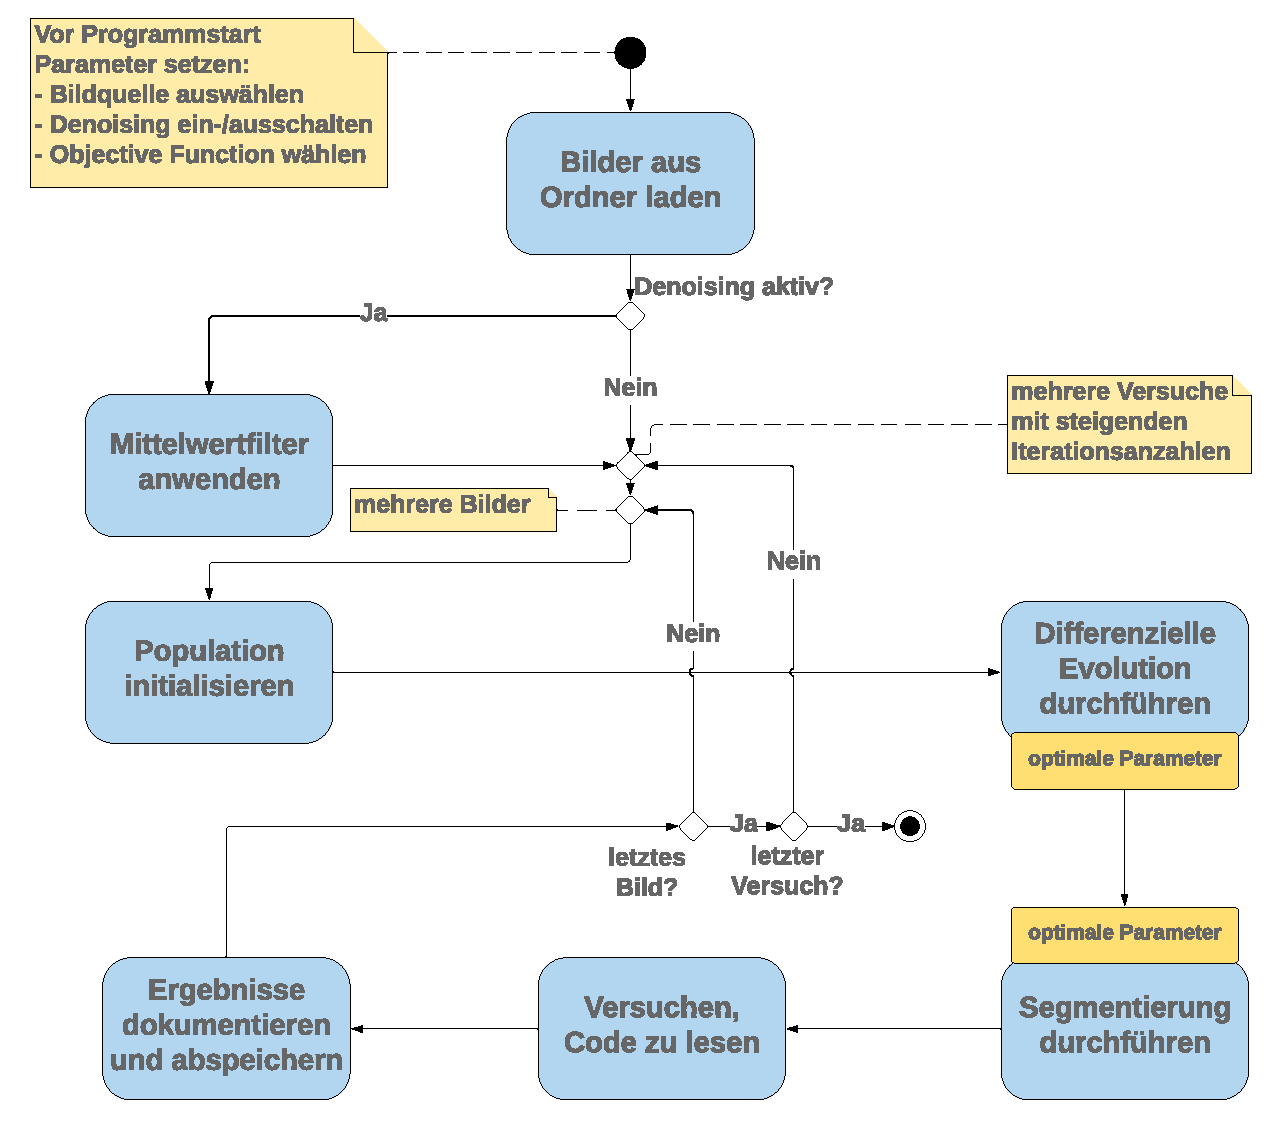
\includegraphics[width=0.9\linewidth]{diff-evol-activity}
				\caption{Aktivitätsdiagramm des Ablaufs in der Test-Applikation}
				\label{fig:diff-evol-activity}
			\end{figure}
			Aus Abbildung \ref{fig:diff-evol-activity} lassen sich die Abläufe entnehmen, die im während dieser Arbeit entwickelten Test-Programm abgehandelt werden.\\
			Vor dem Programmstart müssen unter anderem 
	
		\subsection{Wahl der Programmiersprache}
		\label{sub:prog-lang}
			Auf dem Gebiet der Bildverarbeitung haben sich im Allgemeinen zwei Programmiersprachen bewährt - \textit{Python} und \textit{C++} - nicht zuletzt wegen der in der Praxis oft verwendeten Open-Source-Bibliothek \textit{OpenCV}, die für diese beiden Sprachen eine Anwendungsschnittstelle bereitstellt (siehe Online-Dokumentation). Für diese Arbeit ist die Wahl auf die Sprache Python gefallen, da sie gegenüber C++ einige Vorteile mit sich bringt \cite[S. 21f]{python-book}:\\
			Es bietet erhöhte Lesbarkeit sowie Benutzbarkeit aufgrund der Loslösung von der darunterliegenden physischen Schicht. Oft beträgt der Umfang eines Python-Skripts lediglich bis zu einem Drittel der Größe eines äquivalenten C++-Programms. Somit lassen sich mit Python auch komplexere Applikationen in einem kürzeren Zeitrahmen erstellen als mit C++.

		\subsection{Benutzte Module}
		\label{sub:used-modules}
		
	\section{Ergebnisse}
	\label{sec:results}
	
		\subsection{Vergleich Modell 1 - Modell 2}
		\label{sub:comp-m1-m2}
		
		\subsection{Vergleich unterschiedlicher Bildgruppen}
		\label{sub:comp-diff-images}
		
		\subsection{Einfluss von Denoising auf das Ergebnis}
		\label{sub:influence-of-denoising}
		
		\subsection{Beurteilung des Ergebnisses bei steigender Iterationszahl}
		\label{sub:judging-higher-iteration}